%
% File acl2013.tex
%
% Contact  navigli@di.uniroma1.it
%%
%% Based on the style files for ACL-2012, which were, in turn,
%% based on the style files for ACL-2011, which were, in turn, 
%% based on the style files for ACL-2010, which were, in turn, 
%% based on the style files for ACL-IJCNLP-2009, which were, in turn,
%% based on the style files for EACL-2009 and IJCNLP-2008...

%% Based on the style files for EACL 2006 by 
%%e.agirre@ehu.es or Sergi.Balari@uab.es
%% and that of ACL 08 by Joakim Nivre and Noah Smith

\documentclass[11pt]{article}
\usepackage{acl2013}
\usepackage{times}
\usepackage{url}
\usepackage{latexsym}
\usepackage[pdftex]{graphicx}
\usepackage{subfig}
%\setlength\titlebox{6.5cm}    % You can expand the title box if you
% really have to

\title{Adapting DCS-Trees for Wide-Domain Semantic Parsing}

\author{Amelia Harrison \\
  Department of Computer Science\\
  University of Texas at Austin \\
  {\tt ameliaj@cs.utexas.edu} \\\And
  Subhashini Venugopalan \\
  Department of Computer Science\\
  University of Texas at Austin \\
  {\tt vsubhashini@cs.utexas.edu} \\}

\date{}

\begin{document}
\maketitle
\begin{abstract}
   Recent work in semantic parsing for compositional question answering has shown
that this task can be successfully approached using question-answer pairs rather
than questions annotated with logical forms for training. However, existing
datasets for this task are relatively small and it is unclear that even in
absence of the burden of producing logical forms for training, that any existing
approaches to compositional question answering can scale to larger datasets or
datasets with wide coverage.  In this paper, we explore the possibility of scaling 
one such approach to a larger dataset with wider coverage. 

\end{abstract}

\section{Introduction}

In \cite{LJK11}, Liang et al. present a novel approach to the semantic parsing
task. Most prior approaches have focused on training parsing models using natural
language utterances annotated with logical forms.\footnote{\cite{CGCR10}, 
\cite{CGRR11}, and \cite{PD09} are notable exceptions.} In this work, however,
the logical forms are treated as latent variables, and a semantic parsing model
is trained using natural language questions and their corresponding answers. 
This sort of ``weak supervision'' is advantageous because obtaining 
logical forms for natural language utterances requires expert annotators and is
thus quite costly. This work is notable because it takes this weakly supervised 
approach, and also because it introduces an new formalism called
dependency-based compositional semantics (DCS) trees for representing 
the meaning of a natural language question. In this note, we will briefly
summarize the work in \cite{LJK11}, and suggest some useful ways in which that work
may be extended. 

Recent work has shown that the compositional question answering
task can be successfully approached using question-answer pairs for training
rather than questions annotated with logical forms \cite{LJK11} \cite{}. In
\cite{LJK11},   

\section{Experimental Evaluation}
This section describes the datasets used to evaluate our methods and the results obtained.

\subsection{Data}
We tested our approach on two datasets. The first is the standard {\sc GEO} dataset \cite{ZM96}. To test the scalability of our approach we also create a wide domain dataset by extracting data from DBpedia \cite{dbpedia}. %\cite{dbpedia full link} 
%http://dbpedia.org/Datasets
%http://wiki.dbpedia.org/Downloads38
The DBpedia data set consists of a multi-domain ontology derived from Wikipedia. Our project uses the DBpedia Infobox dataset \cite{dbpedia2, dbInfo} which contains specific facts about things (such as people, places, films, music, books, games) in Wikipedia articles. The Infobox data consists of
\begin{itemize}
\item Type information of the instances in wikipedia such as city, disease, computer game etc.
\item Properties of the instances e.g. population of a city, date of birth.
\item Specific properties specialized for some property value such as units of measurement for a person's height.
\end{itemize}
We build our DBpedia data set by extracting type and property information of all instances (as tuples - describe). This results in a large dataset of unary and binary predicates consisting of over five million facts. 

\paragraph{Relevant wide-domain dataset} We reduce the initial large dataset (DBP) to a more relevant smaller dataset consisting of 538,821 facts. To create this subset, we first considered all the binary predicates in the initial dataset (of the form predicate( key, value) ). Next, we identify all items occuring as a key. We then count the frequency of occurence of each of these items as a value in the tuple and rank and pick the top 30000 most frequent items. We finally select all tuples containing any of these top items as a key. The idea is to select those items that are popular in the database and hence likely to also be more relevant.

\subsection{Methodology}
We evaluate our approach of generating lexical triggers with the DCS framework on the {\sc GEO} dataset as outlined below. We split our evaluation into the following four categories:
\begin{itemize} \label{cats}
 \item $ours$ - Lexical triggers generated purely from our approach. 
 \item $+bridge$ - In addition to our trigger set, we add a small set of bridge predicate triggers described in \cite{LJK11}. (expand?) 
 \item $+general$ - This includes a set of handcoded a general trigger set of lexicons for mathematical operations such as sum and argmax (along with our triggers)
 \item $all$ - The final set of triggers include all of the above, namely, our lexical triggers, the bridge predicate triggers and the general handcoded trigger set.
\end{itemize}
We split the lexical sets into the above categories for triggers generated using wordnet and wackypedia. In all the experiments, the training set consisted of 600 questions and the test set consisted of 280 questions.

\paragraph{Impact of number of lexical triggers per predicate.} We further performed a series of tests to identify if the number of lexical triggers per predicate affected the performance in any way. This test was performed only on the lexical trigger set generated from wackypedia since the context lexical words have a total ordering (rank) and also because this set gave us the best performance. In our experiments we varied the number of lexical words from 1 to 12 and compared the performance of the DCS framework on the four categories described in \ref{cats}.

\section{Results}
\begin{center}
\begin{table}[!h]
\centering
\begin{tabular}{|l|c|c|}
\hline
{\textbf{Lexicon Source}} & {\textbf{WordNet} } & {\textbf{Wackypedia}} \\ %\cline{4}
\textbf{Category}&  & (threshold=6) \\
%\textbf{Function}& (after iteration 8) &\textbf{words}  & (total)\\
\hline
ours     & 0.00 & {{21.78}} \\ \hline
+bridge  & 43.21 & {{42.5}} \\ \hline
+general & 0.00 & {{36.07}} \\ \hline
all      & 61.07 & {\textbf{69.64}} \\ \hline
\end{tabular}
\caption{Comparing performance of external lexical trigger sources on GEO dataset (600 train and 280 test queries)} \label{tab:normal}
\end{table}
\end{center}

\begin{figure}[!htb]
\begin{center}
  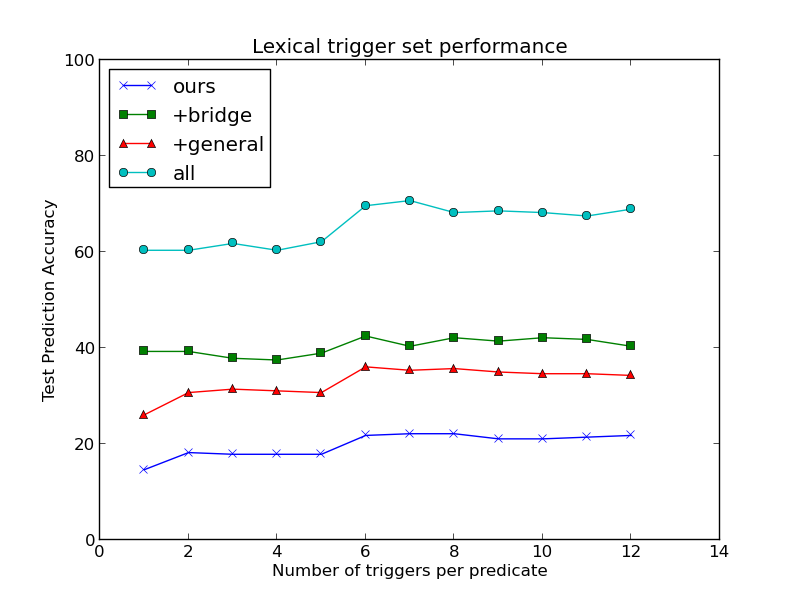
\includegraphics[scale=0.45]{figs/ablationTest.png}
\caption{Graph showing the effect of varying the number of lexical triggers per predicate on GEO.}
\end{center}
\end{figure}

\begin{figure}[!htb]
\begin{center}
  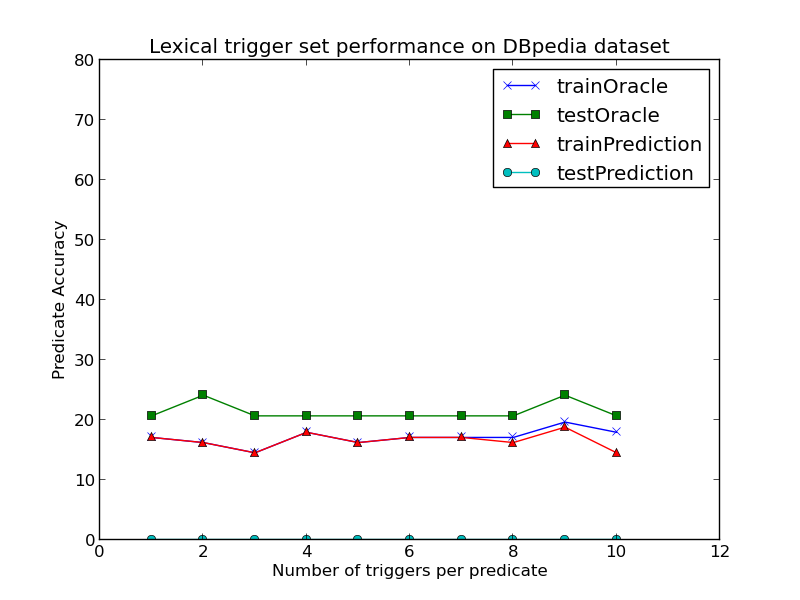
\includegraphics[scale=0.45]{figs/ibPerf.png}
\caption{Performance of automatically generated lexical triggers on the wide-domain DBP dataset (80-20 split).}
\end{center}
\end{figure}

\section{Related Work}
The task of semantic parsing has been studied quite extensively. Early works \cite{ZM96} introduced a statistical approach to learn a semantic parser using inductive logic programming. This led to a line of machine learning approaches \cite{TM01, GeM05, KWM05, ZC07, WM06, KZGS10} that have continually improved the accuracy of semantic parsing.
Although the statistical methods are robust and portable, a major drawback of the approach is that it relies crucially on having natural language utterances paired with their logical forms. This not only requires substantial human effort but also expects the annotators to have expertise in some formal language.

In order to alleviate the burden of annotation recent works \cite{CGRR11, CGCR10, PD09, LJK11, AZ11} %reduce the burden of annotation significantly by obviating the need for logical form annotations and focus on learning from question and answer pairs. 
are focusing on learning directly from question and answer pairs obviating the need for logical forms.


\cite{CGCR10, CGRR11} use external world context to supervise semantic interpretation. Similar in vein to \cite{CM08, LJK09}, the \cite{CGCR10} model learns to map lexical elements to logical forms based on external sources and additionally creates the logical form query relying on the composition rules of the meaning representation language. However, their main contribution that obviates annotated logical forms is the feedback based approach that guides the learning algorithm in identifying hidden alignments between lexical and logical elements.

An important limitation of the \cite{CGCR10} system is that although it does require explicit logical form annotations, their model still relies on the framework of the meaning representations language which lacks in its expressiveness (in its ability to express) natural language queries. Researchers have, in the past, explored widely with respect to the formal language used for the logical forms: \cite{GM09} use SQL, \cite{ZM96,TM01} use prolog, \cite{KWM05}  develop a simple functional query language called {\sc FUN}QL, and \cite{ZC05} use lambda calculus. The construction mechanisms that generate these logical forms in a compositional manner from the utterances have also been quite diverse. The logical forms and the construction mechanisms are in sort of orthogonal problems and hence the expressiveness of these models vary to a good degree.

\cite{LJK11} proposes the DCS trees logical form that pushes towards a deeper representation of language. %Each natural language question
We have discussed the DCS framework previously in [ ref the background]
As mentioned before, although the DCS framework appears to be a good candidate to tackle wide-domain semantic parsing, the model requires some non-trivial supervision to identify the set of lexical triggers.
Our work addresses the task of automatically identifying the lexical triggers in the DCS framework and aims to reduce the burden of supervision further.

Apart from generating the lexical triggers automatically from the database, our work is amongst the first (to the best of our knowledge) to explore the idea of semantic parsing on a wide-domain dataset. The system {\sc BOXER} developed by JB is a wide-coverage semantic parsing system. However, his system is incomparable to our -- due to the lack of evaluation



\section{Other Issues}

Those papers that had software and/or dataset submitted for the review process
should also submit it 
with the camera-ready paper. Besides, the software and/or dataset should not be
anonymous. 

Please note that the publications of ACL 2013 will be publicly available at ACL
Anthology 
(http://aclweb.org/anthology-new/) on July 28th, 2013, one week before the start
of the conference. 
Since some of the authors may have plans to file patents related to their papers
in the conference, 
we are sending this reminder that July 28th, 2013 may be considered to be the
official publication date, 
instead of the opening day of the conference.

\section*{Acknowledgments}

Thanks to Karl Pichotta and Ray Mooney for helpful discussions and healthy
skepticism.

\bibliographystyle{acl}
report.bib
\bibliography{acl2013}


\end{document}
